\section{Outline of baryogenesis}
One way to describe the observed baryonic asymmetry is by a postulating, that the universe has been in an asymmetric state just from the beginning and that the matter and antimatter is concentrated in big domains throughout the universe, which come into contact just at their outer borders. Techincally there is no reason for the universe not to have started in an asymmetric state, in that case one would measure high gamma rates due to the matter-antimatter-annihilation right between these distinct regions. \newline
Since there is no kind of such radiation seen, patches of diffrent kinds of matter have to be as big as the presently observable universe. Because this doesn't seems very plausible, so the baryonic asymmetry had to arise dynamically from an universe where matter and antimatter existed in the same amounts. \newline
Actually in 1967 the Sovjetian physicist Andrei Sakharov postulated the criteria, which have to be met in order for an excess of baryons over anti-baryons to be generated out a fully symmetrical universe.
\subsection{Sakharov Conditions}
As mentioned above there are three crucial properties of nature, the Sakharov conditions, wich are required to produce an net baryon number greater than zero. These three conditions are:
\begin{enumerate}
	\item B-violating process(es)
	\item C and CP violation
	\item Departure from or loss of thermal equilibrium
\end{enumerate}
For an general insight of these three conditions the first one will be skipped, since it is quite obvious, that in an totally symmetric universe there has to be at least one B-violating process in order to cause an inbalance in matter and antimatter. \newline
The general importance of the other two will be discussed in the following.
\subsubsection{C and CP-violation}
Charge conjugation (C), parity (P) and their combination (CP) are two or more specifically three basic symmetries of the universe. C symmetry states, that physical processes are the same, even after exchanging particles for their respective anti-particles, while P-symmetry guarantees invariance under the transformation $\vec{r}\rightarrow-\vec{r}$. CP symmetry then simply is an sequence of a C followed by a P transformation. \newline
To explain why C has to be violated for baryogenesis beeing possible, consider the B-violating reaction
\begin{equation*}
	X\rightarrow Y+B
\end{equation*}
with X and Y particles with B=0 and B representing the excess baryons. This reactions happens with a certain rate, which is, using C as a symmetry, just the same as the reation rate for the conjugate process.
\begin{equation}
	\Gamma(X\rightarrow Y+B)=\Gamma(\bar{X}\rightarrow \bar{Y}+\bar{B})
	\label{c-violation}
\end{equation}
Eq. \ref{c-violation} implies, that under C exactly the same amount of baryons and anti-baryons will be produced and therefore no excess baryons are left after the annihilaton. This means C must be violated. \newline
But additionally to this CP violation is essential for baryogenesis. To illustrate why, take a closer look at the also clearly B  violating X decay with its two channels:
\begin{align*}
	X\rightarrow q_Lq_L\\
	X\rightarrow q_Rq_R
\end{align*}
with q an arbritrary quark. The subscripts L and R denote the the left - or right-handedness chirality of the decay products. CP then effects each particle as follows
\begin{align*}
	X\underset{CP}{\longrightarrow}\bar{X}\\
	q_{L}\underset{CP}{\longrightarrow}\bar{q}_{R}\\
	q_{R}\underset{CP}{\longrightarrow}\bar{q}_{L}
\end{align*}
So CP doesn't just change matter for anti-matter, but the handedness of the particles as well. So if CP holds as a symmetry the consequences for the reaction rates are:
\begin{equation*}
	\Gamma(X\rightarrow q_Lq_L)=\Gamma(\bar{X}\rightarrow \bar{q}_R\bar{q}_R)\hspace{2cm}\Gamma(X\rightarrow q_Rq_R)=\Gamma(\bar{X}\rightarrow \bar{q}_L\bar{q}_L)
\end{equation*}
Adding these two results in 
\begin{equation}
\Gamma(X\rightarrow q_Lq_L)+\Gamma(X\rightarrow q_Rq_R)=\Gamma(\bar{X}\rightarrow \bar{q}_R\bar{q}_R)+\Gamma(\bar{X}\rightarrow \bar{q}_L\bar{q}_L)
\label{cp-violation}
\end{equation}
Eq. \ref{cp-violation} implies, that as long as there are as many particles X as anti-particles $\bar{\text{X}}$ in the initial state of the universe, which is just the starting point of the modell the Sakharov conditions try to describe, there can only be an asymmetry between left and right-handed particles be achieved, but that isn't a baryon asymmetry, which is clearly needed for baryogenesis. CP must be violated.\newline
So the bottom line here is, that the existence of B-violating processes is not sufficient for baryogenesis, but that there also has to be C and also CP violation, since without this kind of symmetry breaking any baryonic excess would be washed out by the corresponding C or CP conjugated process, as shown with the simple examples above. 
\subsubsection{Departure from thermal equilibrium}
The last condition to be met in order for baryogenesis to be achievable is that the the B, C and CP violating processes must occur outside the thermal equilibrium. To illustrate this we first consider the phase space distribution of a species X of quantum particles
\begin{equation}
	f(E_X)=\frac{1}{e^{\frac{E_X-\mu_X}{T}}\pm1}
	\label{distribution}
\end{equation}
The energy E$_X$ and the momentum $\vec{p}_X$ are related via the relativistic energy-momentum-relation $E^2=\vec{p}^2+m^2$. $\mu_X$ describes the chemical potential of the particle species X, which is an important quantity for describing thermal equilibrium states, as the chemical potentials of two species X and Y, which are in thermal equilibrium are related by $\mu_X=\mu_Y$ or for more species $\sum_i\mu_i=0$.\newline
Using eq. \ref{distribution} to compute the particle density of a certain particle species one gets 
\begin{equation}
	n_X=g_X\int\frac{d^3p}{(2\pi)^3}\:f_X(E)
	\label{density_n}
\end{equation}
where g$_X$ denotes the number of inner degrees of freedom of X. \newline
In the non-relativistic limit there holds m $\gg$ E-$\mu\gg$ T. With this approximation the denominator of the exponential function in eq. \ref{distribution} gets small compared to the numerator so the exponential itself gets so big that the $\pm$1 can be neglected, in the non-relativistic limit, you get the same particle density for fermions and bosons. By dividing the ernergy E$_X$ into the rest energy m$_X$ and the kinetic energy E$_{\text{kin}}$ and after approximating
\begin{equation}
	E_{\text{kin}}\approx\frac{p^2}{2m}
\end{equation}
for non-relativistic particles, integrating according to \ref{density_n} yields
\begin{equation}
n_X=g_X\frac{4\pi}{(2\pi)^3}\int dp\:p^2e^\frac{\mu-m_X}{T}e^{-\frac{p^2}{2m_XT}}=g_X\left(\frac{m_XT}{2\pi}\right)^\frac{3}{2}e^{-\frac{m_X-\mu_X}{T}}
\label{numerX}
\end{equation}
Analogously you get the number density for the corresponding anti-particle $\bar{\text{X}}$
\begin{equation}
	n_{\bar{X}}=g_{\bar{X}}\left(\frac{m_{\bar{X}}T}{2\pi}\right)^\frac{3}{2}e^{-\frac{m_{\bar{X}}-\mu_{\bar{X}}}{T}}
\label{numberantiX}
\end{equation}
Now suppose X and its anti-particle $\bar{\text{X}}$  with B$_X=-$B$_{\bar{X}}\neq0$ are in thermal equilibrium than the condition $\mu_X=\mu_{\bar{X}}$ holds. Comparing eq. \ref{numerX} and \ref{numberantiX} one sees, that the chemical potential is the only property that could differ for particles and antiparticles. Now using the equilibrium condition for chemical one finally gets
\begin{equation}
	n_X=n_{\bar{X}}
	\label{thermalequ}
\end{equation}
Looking at eq \ref{thermalequ} it is quite obvious that even with B, C and CP violating any produced excess baryon number B will be washed out in equilibrium by other processes happening in equilibrium. \newline
This illustrates the final Sakharov Condition, that next to B, C and CP violation a departure from equilibrium is needed for a dynamic production of excess baryons. \newline
Interresting to note is, that there is quite an easy way of approximatelly determining if reactions take place in thermal equilibrium is by comparing the reaction rate with the expansion of universe, discribed by the Hubble constant H, which isn't actually a constant but changes with time. So if the relation 
\begin{equation}
	\Gamma\gtrsim H
	\label{rate_g_hubble}
\end{equation}
holds, the reactions take place fast enough for them to be in equilibrium. This can be made understandable, it is useful to look at this from the rest fram of the particles taking part in the reactions. Then the particles don't notice any expansion of the universe since they move and react to fast with each other, therefore the expansion doesn't really affect the equilibrium state. \newline
Otherwise if the reactions occur slower than the universe expands, so if 
\begin{equation}
	\Gamma<H
\end{equation}
is valid, than the expansions happens fast enough that particles get separated too far from each other, so they can't react anymore and the reactions fall out of equilibrium.
\subsection{Baryogenesis in the Standard Modell}
Although nowadays there are no records or experimental proofs of baryon number violating processes, that doesn't mean there is a need for physics outside the Standard Modell (SM) of particle physics, at least on a qualitative level.
\subsubsection{Electroweak baryogenesis}
As it turns out the electroweak part of the SM with its SU(2)$_L\times$U(1)$_Y$ symmetry groups suits best for describing baryogenesis. The following discussions will illustrate how the SM satisfies all three Sakharov conditions.\newline
\paragraph{C and CP violation}
It is already proven theoretically und experimentally by numerous well-known experiments, like for example the Wu experiment in 1956, that C symmetry is maximally violated by the weak interaction in the leptonic as well as in the hadronic sector. As shown by Kobayashi and Maskawa through expanding the Cabibbo hypothesis and experimentally confirmed, weak interactions in the hadronic sector also violate CP invariance, which manifests as an complex phase in the CKM quark mixing matrix. In the leptonic sector however the CP violation through a complex phase only got postulated in the PMNS neutrino mixing matrix to try to descripe neutrino oscillations, but this phase still needs to be measured.\newline
Nevertheless the elektroweak part of the SM, more precise the weak interactions, since electromagnetism doesn't violate C or even P, satisfies at least one of the three Sakharov conditions.\newline
\paragraph{B violation}
Although the first Sakharov condition, the necessity of baryon number violating processes, seems to be the most obvious, the way these are realised in the SM is a bit more difficult than it seems. \newline
Since at the first look the baryonic and, since it is going to play an important role during the following discussion, the leptonic current are  conserved
\begin{align}
	\partial^\mu J_\mu^B=0
	\label{Bcurrent}
	\\
	\partial^\mu J_\mu^L=0
	\label{Lcurrent}
\end{align}
one would assume there is no way the SM could produce an baryon asymmetry. However, by considering quantum fluctuation meaning orders higher than just tree level one finds, that the currents for the left- and right-handed parts f$_L$ and f$_R$ respectively, where stands for quarks and leptons equally, aren't conserved and not the same \cite{Bernreuther:2002uj}
\begin{align}
	\partial^\mu\bar{f}_L\gamma_\mu f_L&=-c_L\frac{g^2}{32\pi^2}F^a_{\mu\nu}\tilde{F}^{a\mu\nu}
	\label{l_chiralty_current}
	\\
	\partial^\mu\bar{f}_R\gamma_\mu f_R&=+c_R\frac{g^2}{32\pi^2}F^a_{\mu\nu}\tilde{F}^{a\mu\nu}
	\label{r_chiralty_current}
\end{align}
where g denotes the gauge coupling, F$^{a\mu\nu}$ the field tensor, $\tilde{F}^{a\mu\nu}$ the dual field tensor and c$_L$ and c$_R$ depend on the representation of f$_L$ and f$_R$.This behaviour of the currents at quantum levels is known as Adler-Bell-Jackiw or chiralty anomaly. 
Since SU(2)$_L$ gauge boson only couples with left-handed particles c$_R^W$=0, while the U(1)$_Y$ gauge boson couples to both hadednesses, but with different strength, therefore c$_R^Y\neq$c$_L^Y$. Although this section only focuses on electroweak baryogenesis, it is mentionable that with the SU(3)$_c$ gauge bosons of the strong interactions don't produce any chiralty anomaly because they couple with left as well as right-handed particles with the same strenght, so c$_R^c=$c$_L^c$ and both currents in \eqref{l_chiralty_current} and \eqref{r_chiralty_current} cancel each other out in the case of strong interactions. \newline
Putting this and eqautions \ref{Bcurrent} - \ref{r_chiralty_current} together, gives a pretty interesting result
\begin{equation}
\partial^\mu J_\mu^B=\partial^\mu J_\mu^L=\frac{n_F}{32\pi^2}\left(-g_w^2W^a_{\mu\nu}\tilde{W}^{a\mu\nu}g'^2G^a_{\mu\nu}\tilde{G}^{a\mu\nu}\right)
\label{B-L}
\end{equation}
with W$^{a\mu\nu}$ and B$^{a\mu\nu}$ the field strenght tensors of the SU(2)$_L$ and U(1)$_Y$ gauge groups and n$_F$=3 the number of particle families. \newline
Analyzing eq. \ref{B-L} one easily figures out, that although baryon and lepton number are not conserved separatedly the difference B-L of these numbers is very well conserved.
Integrating both sides of eq. \ref{B-L} as shown in \cite[pp. 15-16]{Bernreuther:2002uj} results in 
\begin{equation}
	\Delta B=\Delta L=n_F\Delta N_{CS}
	\label{number_change}
\end{equation}
where $\Delta$N$_{CS}$ is the difference of so called Chern-Simons numbers. How exatly these numbers are derived and what there integral representation is can also be looked up in \cite{Bernreuther:2002uj,Cline:2006ts,Petropoulos:2003pm}, but isn't of great interest for this thesis. However one property of these numbers is quite relevant for baryon asymmetry, namely that each integer valued Chern-Simons number describes one distinct vacuum state of the infinite electroweak vacua with minimal energy, which are separated by an potential barrier. The difference of these numbers of two vacuum states right next to each other is $\Delta$N$_{CS}=\pm1$, so changing from one vacuum state N$_i$ to another N$_f$ results in $\Delta$N$_{CS}\neq0$ and therefore an change in baryon and lepton number is induced. Also interesting to notice is, since the number of particle families n$_F$=3 baryon and lepton numbers change at least by three units each. \newline
The last question regarding B violation in the SM is about how such a transition between two vacuum states can be accomplished. One way is through a quantummechanical effect called the instaton, where the system simply tunnels through the barrier between to vacuum states with different Cher-Simons numbers. However 't Hooft, the one showing B vioaltion by the chiral anomaly, also showed  \cite[Ref. 22,24]{Bernreuther:2002uj} that the cross section for such a tunneling process is about 
\begin{equation}
	\sigma\propto e^{-\frac{4\pi}{\alpha_w}}\sim10^{-164}
	\label{instaton_cross_section}
\end{equation}
with $\alpha_w=\frac{g^2}{4\pi}\cong\frac{1}{30}$.
This cross section is so small, that such a instaton transition between two vacua probably didn't happen even once during the whole lifetime of the universe. \newline
A second way such an change of vacua can be induced is through the so called sphaleron processes. The requirement for these processes to take place is that the system has enough energy to go over the potential barrier instead of tunneling through. The minimum energy needed, knowon as the spaleron energy, is about\cite{Bernreuther:2002uj,Cline:2006ts}
\begin{equation}
	E_{sph}=\frac{2M_W}{\alpha_W}f\left(\frac{\lambda}{g_W^2}\right)\cong8-13\text{TeV}
	\label{spaleron}
\end{equation} 
where $\lambda$ describes the four-Higgs interaction and the funtion f lives on an intervall [1.56,2.72].\newline
In fact these kind of processes are quite possible for temperatures above around 100 GeV, however below this temperature the rate of spaleron processes is exponentially suppressed by a Boltzmann factor. It is also mentionable that comparing the sphaleron rate for temperatures above 100 GeV, which are proportional to the fourth power of the temperature \cite[p. 19]{Bernreuther:2002uj}, with the Hubble constant, gives information about when these processes are in thermal equilibrium and numerical evaluations yield that the sphaleron processes are in thermal equilibrium for
\begin{equation*}
100\text{GeV}\lesssim T \lesssim 10^{12}\text{GeV}
\end{equation*}
So as shown in section 2.1.2, even though the SM provides the necessary tools for C, CP and B violation, below the temperature of around 10$^{12}$GeV any produced net baryon number will be washed out and below 100 GeV the temperature isn't even high enough to induce sphaleron processes. \newline
\paragraph{Departure from thermal equilibrium and elecroweak phase transistion} The final question to answer regarding baryogenesis in the SM is how the last Sakharov condition, the departure from thermal equilibrium is realized. The most common way is by using the electroweak phase transition. \newline
This phenomenon heavily relies on the vacuum expation value (VEV) of the SU(2)$_L$ Higgs doublett and its behaviour during the early times of the universe. At the present day the VEV isn't equal to zero, which leads to a gauge symmetry breaking and therefore masses of every massive particle. But it has already be shown \cite[Ref. 32]{Bernreuther:2002uj}, that for high temperatures the VEV of the universe equals zero and the SU(2)$_L\times$U(1)$_Y$ gauge symmetry is till intact, even at the ground states. This obviously means, that at some point during the evolution of the universe and at some critical temperature T=T$_c$ the VEV changed from zero to non-zero, or in other words a phase transition from a totally symmetrical phase to a phase with broken symmetry happened at some point. In order to generate a departure from thermal equilibrium for the B vioalating reaction this transition must be strongly of first order, meaning at T=T$_c$ the VEV changes discontinuously from zero to non-zero. \newline
Just as with cooling steam this process can be imagined with bubbles of phases with broken symmetries forming and expanding inside the phase of unbroken symmetry, just as droplets of water form in the vapor and expand, until the connect and finally cover all space. Now the way this phase transition leads to a baryon asymmetry is as follows. \newline
First of all consinder a thin wall, so that the area where quarks and fermions interact with the walls can be approximated as a step function. Also, to simplify matters, assume that the expansion of the bubbles of broken symmetry is sperical symmetric, so this problem can be reduced to one dimension. \newline
At the start of this baryon asymmetry generating process there is the same amount of particles and anti-particles. \newline
While the bubble expands left- and right-handed quarks and anti-quarks from the unbroken phase hit the bubble wall, get reflected under CP violating processes and change their handedness because of angular momentum conservation and since charge conservation holds (anti-)quarks are only allowed to scatter into (anti-)quarks. The scattering processes are the following
\begin{align*}
	q_L\rightarrow q_R\\
	q_R\rightarrow q_L\\
	\bar{q}_L\rightarrow \bar{q}_R\\
	\bar{q}_L\rightarrow \bar{q}_R
\end{align*}
Since these scattering processes are not CP conserving the reflection coefficents are not the same for all of the reactions above.
\begin{equation}
	\Delta R=R_{\bar{L}\rightarrow\bar{R}}-R_{R\rightarrow L}=R_{\bar{R}\rightarrow\bar{L}}-R_{L\rightarrow R}
	\label{reflection_coeff}
\end{equation}
Using CPT invariance yields
\begin{align}
	R_{\bar{L}\rightarrow\bar{R}}=R_{L\rightarrow R}\\
	R_{\bar{R}\rightarrow\bar{L}}=R_{R\rightarrow L}
\end{align}
These relations alone imply that there still is no net baryon number since the differences J$^L_q$ of the fluxes of $\bar{q}_R$ and q$_L$ and the  J$^R_q$ of q$_R$ and$\bar{q}_L$ reflected back into the symmetric phase are the same and cancel each other out. But considering that the (B+L) violating sphaleron processes because of their electroweak origin only interact with left-handed quarks and right-handed anti-quarks J$^L_q$ changes while  J$^R_q$ stays the same since it only takes right-handed quarks and left-handed antiquarks into account. This leads to a non-zero baryon number and especially if  J$^L_q$>0 than there are more left-handed quarks then right-handed anti-quarks and therefore $\Delta$B>0 in the symmetric phase away from the wall. If the bubble than expands over the region of a net baryon number greater zero this B gets frozen in, since in the broken phase the (B+L) violating processes that could wash out the asymmetry are strongly supressed by the Boltzmann factor as stated above. \newline
Taking into account that particles from the broken phase can transmit into the symmetric phase and evaluating this quantitative as shown in \cite[pp. 36-37]{Bernreuther:2002uj} yields the result mentioned above. For an net baryon number greater than zero the CP violating processes at the bubble wall have to act in such way that the current J$^L_q$ is greater than zero as well. 
\subsubsection{Failures of the SM}
Since the SM offers everything needed to describe baryogenesis in the early universe one could naively say that the only thing left is the experimental proof to be delivered. \newline
Having said this recent experiments have shown that the SM alone, despite containing possible B, C and CP violating processes, isn't able to provide an phase transition of strong enough first order or more precisely a phase transition of first order at all. 
\begin{figure}[H]
	\centering
	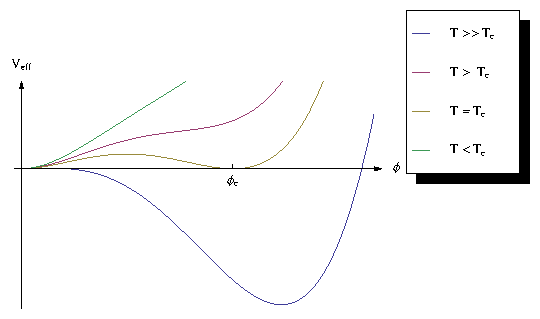
\includegraphics[width=0.7\linewidth]{Images/Higgs}
	\caption{Effective Higgs potential for different temperatures in case of a first order phase transition}
	\label{fig:higgs}
\end{figure}


%%% mode: latex
%%% TeX-master: "../Leptogenesis"
%%% End: